\documentclass[twoside]{book}

% Packages required by doxygen
\usepackage{fixltx2e}
\usepackage{calc}
\usepackage{doxygen}
\usepackage[export]{adjustbox} % also loads graphicx
\usepackage{graphicx}
\usepackage[utf8]{inputenc}
\usepackage{makeidx}
\usepackage{multicol}
\usepackage{multirow}
\PassOptionsToPackage{warn}{textcomp}
\usepackage{textcomp}
\usepackage[nointegrals]{wasysym}
\usepackage[table]{xcolor}

% Font selection
\usepackage[T1]{fontenc}
\usepackage[scaled=.90]{helvet}
\usepackage{courier}
\usepackage{amssymb}
\usepackage{sectsty}
\renewcommand{\familydefault}{\sfdefault}
\allsectionsfont{%
  \fontseries{bc}\selectfont%
  \color{darkgray}%
}
\renewcommand{\DoxyLabelFont}{%
  \fontseries{bc}\selectfont%
  \color{darkgray}%
}
\newcommand{\+}{\discretionary{\mbox{\scriptsize$\hookleftarrow$}}{}{}}

% Page & text layout
\usepackage{geometry}
\geometry{%
  a4paper,%
  top=2.5cm,%
  bottom=2.5cm,%
  left=2.5cm,%
  right=2.5cm%
}
\tolerance=750
\hfuzz=15pt
\hbadness=750
\setlength{\emergencystretch}{15pt}
\setlength{\parindent}{0cm}
\setlength{\parskip}{3ex plus 2ex minus 2ex}
\makeatletter
\renewcommand{\paragraph}{%
  \@startsection{paragraph}{4}{0ex}{-1.0ex}{1.0ex}{%
    \normalfont\normalsize\bfseries\SS@parafont%
  }%
}
\renewcommand{\subparagraph}{%
  \@startsection{subparagraph}{5}{0ex}{-1.0ex}{1.0ex}{%
    \normalfont\normalsize\bfseries\SS@subparafont%
  }%
}
\makeatother

% Headers & footers
\usepackage{fancyhdr}
\pagestyle{fancyplain}
\fancyhead[LE]{\fancyplain{}{\bfseries\thepage}}
\fancyhead[CE]{\fancyplain{}{}}
\fancyhead[RE]{\fancyplain{}{\bfseries\leftmark}}
\fancyhead[LO]{\fancyplain{}{\bfseries\rightmark}}
\fancyhead[CO]{\fancyplain{}{}}
\fancyhead[RO]{\fancyplain{}{\bfseries\thepage}}
\fancyfoot[LE]{\fancyplain{}{}}
\fancyfoot[CE]{\fancyplain{}{}}
\fancyfoot[RE]{\fancyplain{}{\bfseries\scriptsize Generated by Doxygen }}
\fancyfoot[LO]{\fancyplain{}{\bfseries\scriptsize Generated by Doxygen }}
\fancyfoot[CO]{\fancyplain{}{}}
\fancyfoot[RO]{\fancyplain{}{}}
\renewcommand{\footrulewidth}{0.4pt}
\renewcommand{\chaptermark}[1]{%
  \markboth{#1}{}%
}
\renewcommand{\sectionmark}[1]{%
  \markright{\thesection\ #1}%
}

% Indices & bibliography
\usepackage{natbib}
\usepackage[titles]{tocloft}
\setcounter{tocdepth}{3}
\setcounter{secnumdepth}{5}
\makeindex

% Hyperlinks (required, but should be loaded last)
\usepackage{ifpdf}
\ifpdf
  \usepackage[pdftex,pagebackref=true]{hyperref}
\else
  \usepackage[ps2pdf,pagebackref=true]{hyperref}
\fi
\hypersetup{%
  colorlinks=true,%
  linkcolor=blue,%
  citecolor=blue,%
  unicode%
}

% Custom commands
\newcommand{\clearemptydoublepage}{%
  \newpage{\pagestyle{empty}\cleardoublepage}%
}

\usepackage{caption}
\captionsetup{labelsep=space,justification=centering,font={bf},singlelinecheck=off,skip=4pt,position=top}

%===== C O N T E N T S =====

\begin{document}

% Titlepage & ToC
\hypersetup{pageanchor=false,
             bookmarksnumbered=true,
             pdfencoding=unicode
            }
\pagenumbering{alph}
\begin{titlepage}
\vspace*{7cm}
\begin{center}%
{\Large Excellentea \\[1ex]\large 1.\+0 }\\
\vspace*{1cm}
{\large Generated by Doxygen 1.8.15}\\
\end{center}
\end{titlepage}
\clearemptydoublepage
\pagenumbering{roman}
\tableofcontents
\clearemptydoublepage
\pagenumbering{arabic}
\hypersetup{pageanchor=true}

%--- Begin generated contents ---
\chapter{Guidelines}
\label{md_CONTRIBUTING}
\Hypertarget{md_CONTRIBUTING}
This file will contain the main guidelines for contribution to the project. 
\chapter{R\+E\+A\+D\+ME}
\label{md_README}
\Hypertarget{md_README}


\section*{Description}

Excellentea is an automatic tea maker. The user can operate the machine remotely through an online interface. In other words, you can order your tea, by chosing from several modes, as you leave work and find it ready when you get home. It also comes with the option of controlling the machine using control buttons and an L\+CD display.

\section*{Usage}

\subsection*{Installation}

Clone the repository to your Raspberry Pi and run the following commands\+:


\begin{DoxyCode}
./configure
make
make install
\end{DoxyCode}
 The program can then be started by running the command


\begin{DoxyCode}
excellentea
\end{DoxyCode}
 from the terminal.

\subsection*{User operation}


\begin{DoxyEnumerate}
\item Load your cup with water
\item Load your tea infuser with the tea of your choice
\item Activate the tea maker from the online user interface
\item Choose the brewing mode of your tea
\item Wait...tea is ready\+:)
\end{DoxyEnumerate}

\section*{Hardware}

\subsection*{Key components}


\begin{DoxyItemize}
\item 1 Raspberry PI microcontroller board (tested on version 3 Model B)
\item 1 \mbox{\hyperlink{classStepper}{Stepper}} motor (M\+I\+K\+R\+O\+E-\/1530)
\item 1 Digital temperature sensor (ds18b20)
\item 12V DC power supply
\item 1 heating element (12V) (B004\+O8\+B\+G\+XE)
\item 1 tea infuser
\item 1 reed float sensor (59630)
\item 2 18-\/pin through hole socket (E\+D18\+DT)
\item 2 Darlington transistor array (U\+L\+N2803A)
\item L\+CD
\item 2 N-\/channel logic-\/level M\+O\+S\+F\+ET (F\+Q\+P30\+N06L)
\item M\+O\+S\+F\+ET heat sink (507222\+B00000G)
\end{DoxyItemize}

\subsection*{Additional components}

The project also requires standard passive components (e.\+g. resistors), prototyping tools (e.\+g. breadboard/pcb) and materials for the encasing. See the \href{Main.sch}{\tt circuit schematics} for details.

\subsection*{Protocol}

The digital temperature sensor \mbox{\hyperlink{classDS18B20}{D\+S18\+B20}} communicates with the board through a 1-\/wire protocol on pin 7 (B\+C\+M4). The reed float sensor only outputs two-\/states so a communication protocol is not required.

\subsection*{Prerequisites}

The raspberry PI must be connected to the internet for remote access.

\section*{Software}

\subsection*{Flow diagram}



\section*{Authors}


\begin{DoxyItemize}
\item \href{https://github.com/andreaspanou}{\tt {\bfseries Andrea Spanou}} -\/ {\itshape Initial work}
\item \href{https://github.com/CiaranAnthony}{\tt {\bfseries Ciaran Mc\+Geady}} -\/ {\itshape Initial work}
\item \href{https://github.com/SimoneMarcigaglia}{\tt {\bfseries Simone Marcigaglia}} -\/ {\itshape Initial work}
\end{DoxyItemize}

See also the list of \href{https://github.com/GlasgowTeam3RTEP/ExcellenTea/contributors}{\tt contributors} who participated in this project.

\section*{Contributing}

Please read \mbox{\hyperlink{md_CONTRIBUTING}{C\+O\+N\+T\+R\+I\+B\+U\+T\+I\+NG.md}} for details on our code of conduct, and the process for submitting pull requests to us.

\section*{License}

This project is licensed under the M\+IT License -\/ see the \mbox{[}L\+I\+C\+E\+N\+SE\mbox{]}(L\+I\+C\+E\+N\+SE) file for details.

\section*{Acknowledgments}

We would like to thank the weather in Glasgow for making us think about tea all the time. 
\chapter{Hierarchical Index}
\section{Class Hierarchy}
This inheritance list is sorted roughly, but not completely, alphabetically\+:\begin{DoxyCompactList}
\item \contentsline{section}{sensor}{\pageref{classsensor}}{}
\begin{DoxyCompactList}
\item \contentsline{section}{ds18b20}{\pageref{classds18b20}}{}
\end{DoxyCompactList}
\item \contentsline{section}{stepper}{\pageref{classstepper}}{}
\item \contentsline{section}{tea}{\pageref{classtea}}{}
\end{DoxyCompactList}

\chapter{Class Index}
\section{Class List}
Here are the classes, structs, unions and interfaces with brief descriptions\+:\begin{DoxyCompactList}
\item\contentsline{section}{\mbox{\hyperlink{classActuator}{Actuator}} \\*A general class for external loads }{\pageref{classActuator}}{}
\item\contentsline{section}{\mbox{\hyperlink{classBrewTimer}{Brew\+Timer}} }{\pageref{classBrewTimer}}{}
\item\contentsline{section}{\mbox{\hyperlink{classControllerThread}{Controller\+Thread}} }{\pageref{classControllerThread}}{}
\item\contentsline{section}{\mbox{\hyperlink{classCppThread}{Cpp\+Thread}} \\*G\+NU G\+E\+N\+E\+R\+AL P\+U\+B\+L\+IC L\+I\+C\+E\+N\+SE Version 3, 29 June 2007 }{\pageref{classCppThread}}{}
\item\contentsline{section}{\mbox{\hyperlink{classCppTimer}{Cpp\+Timer}} }{\pageref{classCppTimer}}{}
\item\contentsline{section}{\mbox{\hyperlink{classDS18B20}{D\+S18\+B20}} \\*Class for the digital temperature sensor \mbox{\hyperlink{classDS18B20}{D\+S18\+B20}} }{\pageref{classDS18B20}}{}
\item\contentsline{section}{\mbox{\hyperlink{classSensor}{Sensor}} \\*A general class for simple H\+I\+G\+H/\+L\+OW sensors }{\pageref{classSensor}}{}
\item\contentsline{section}{\mbox{\hyperlink{classStepper}{Stepper}} \\*A class to control stepper motors }{\pageref{classStepper}}{}
\item\contentsline{section}{\mbox{\hyperlink{classTea}{Tea}} \\*A class defining a type of tea by its brewing time and temperature }{\pageref{classTea}}{}
\item\contentsline{section}{\mbox{\hyperlink{classWebThread}{Web\+Thread}} \\*A thread that handles the web interface }{\pageref{classWebThread}}{}
\end{DoxyCompactList}

\chapter{Class Documentation}
\hypertarget{classActuator}{}\section{Actuator Class Reference}
\label{classActuator}\index{Actuator@{Actuator}}


A general class for external loads.  




{\ttfamily \#include $<$Actuator.\+h$>$}

\subsection*{Public Member Functions}
\begin{DoxyCompactItemize}
\item 
\mbox{\hyperlink{classActuator_a8323c15d7ca85370d2760cbcaba7cb07}{Actuator}} (short G\+P\+IO)
\begin{DoxyCompactList}\small\item\em Class constructor. \end{DoxyCompactList}\item 
\mbox{\Hypertarget{classActuator_a5537adf881ed487909d9c08c5d6aa11c}\label{classActuator_a5537adf881ed487909d9c08c5d6aa11c}} 
virtual void \mbox{\hyperlink{classActuator_a5537adf881ed487909d9c08c5d6aa11c}{initialise}} ()
\begin{DoxyCompactList}\small\item\em Initialisation procedure with the wiring\+Pi library. \end{DoxyCompactList}\item 
\mbox{\Hypertarget{classActuator_ad601cfe00148629da1c4dbbee51bbc8c}\label{classActuator_ad601cfe00148629da1c4dbbee51bbc8c}} 
void \mbox{\hyperlink{classActuator_ad601cfe00148629da1c4dbbee51bbc8c}{switch\+On}} ()
\begin{DoxyCompactList}\small\item\em Sets the value of the pin to H\+I\+GH. \end{DoxyCompactList}\item 
\mbox{\Hypertarget{classActuator_a4ba3e5924188bb4f9f81a5adebb70be5}\label{classActuator_a4ba3e5924188bb4f9f81a5adebb70be5}} 
void \mbox{\hyperlink{classActuator_a4ba3e5924188bb4f9f81a5adebb70be5}{switch\+Off}} ()
\begin{DoxyCompactList}\small\item\em Sets the value of the pin to L\+OW. \end{DoxyCompactList}\end{DoxyCompactItemize}


\subsection{Detailed Description}
A general class for external loads. 

This class merely allows the H\+I\+G\+H/\+L\+OW switching of pins ideal for external loads connected through logic-\/level M\+O\+S\+F\+E\+Ts/transistor. 

\subsection{Constructor \& Destructor Documentation}
\mbox{\Hypertarget{classActuator_a8323c15d7ca85370d2760cbcaba7cb07}\label{classActuator_a8323c15d7ca85370d2760cbcaba7cb07}} 
\index{Actuator@{Actuator}!Actuator@{Actuator}}
\index{Actuator@{Actuator}!Actuator@{Actuator}}
\subsubsection{\texorpdfstring{Actuator()}{Actuator()}}
{\footnotesize\ttfamily Actuator\+::\+Actuator (\begin{DoxyParamCaption}\item[{short}]{G\+P\+IO }\end{DoxyParamCaption})}



Class constructor. 


\begin{DoxyParams}{Parameters}
{\em G\+P\+IO} & Raspberry pi pin connected to the actuator. \\
\hline
\end{DoxyParams}


The documentation for this class was generated from the following files\+:\begin{DoxyCompactItemize}
\item 
Classes/Actuator.\+h\item 
Classes/Actuator.\+cpp\end{DoxyCompactItemize}

\hypertarget{classBrewTimer}{}\section{Brew\+Timer Class Reference}
\label{classBrewTimer}\index{Brew\+Timer@{Brew\+Timer}}


Inheritance diagram for Brew\+Timer\+:\nopagebreak
\begin{figure}[H]
\begin{center}
\leavevmode
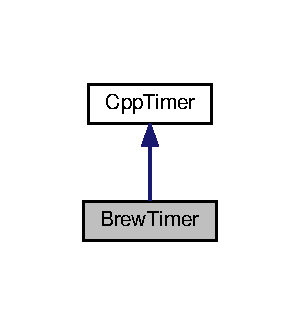
\includegraphics[width=144pt]{classBrewTimer__inherit__graph}
\end{center}
\end{figure}


Collaboration diagram for Brew\+Timer\+:\nopagebreak
\begin{figure}[H]
\begin{center}
\leavevmode
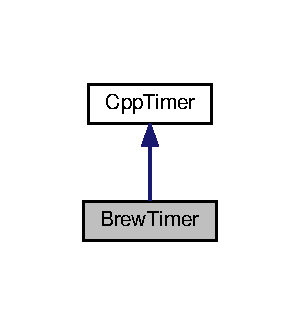
\includegraphics[width=144pt]{classBrewTimer__coll__graph}
\end{center}
\end{figure}
\subsection*{Additional Inherited Members}


The documentation for this class was generated from the following file\+:\begin{DoxyCompactItemize}
\item 
Classes/Brew\+Timer.\+h\end{DoxyCompactItemize}

\hypertarget{classControllerThread}{}\section{Controller\+Thread Class Reference}
\label{classControllerThread}\index{Controller\+Thread@{Controller\+Thread}}


Inheritance diagram for Controller\+Thread\+:\nopagebreak
\begin{figure}[H]
\begin{center}
\leavevmode
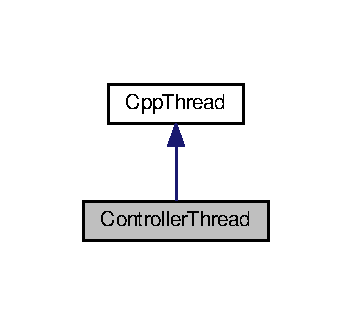
\includegraphics[width=169pt]{classControllerThread__inherit__graph}
\end{center}
\end{figure}


Collaboration diagram for Controller\+Thread\+:\nopagebreak
\begin{figure}[H]
\begin{center}
\leavevmode
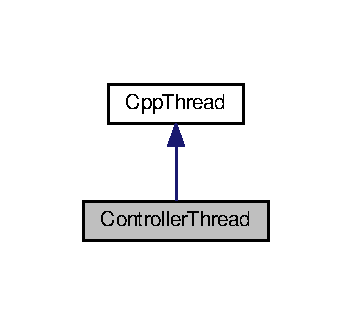
\includegraphics[width=169pt]{classControllerThread__coll__graph}
\end{center}
\end{figure}
\subsection*{Public Member Functions}
\begin{DoxyCompactItemize}
\item 
\mbox{\Hypertarget{classControllerThread_a00cd6502504f5f1e680e6be3f60a987d}\label{classControllerThread_a00cd6502504f5f1e680e6be3f60a987d}} 
\mbox{\hyperlink{classControllerThread_a00cd6502504f5f1e680e6be3f60a987d}{Controller\+Thread}} ()
\begin{DoxyCompactList}\small\item\em Class constructor. \end{DoxyCompactList}\end{DoxyCompactItemize}


The documentation for this class was generated from the following files\+:\begin{DoxyCompactItemize}
\item 
Classes/Controller\+Thread.\+h\item 
Classes/Controller\+Thread.\+cpp\end{DoxyCompactItemize}

\hypertarget{classCppThread}{}\section{Cpp\+Thread Class Reference}
\label{classCppThread}\index{Cpp\+Thread@{Cpp\+Thread}}


G\+NU G\+E\+N\+E\+R\+AL P\+U\+B\+L\+IC L\+I\+C\+E\+N\+SE Version 3, 29 June 2007.  




{\ttfamily \#include $<$Cpp\+Thread.\+h$>$}



Inheritance diagram for Cpp\+Thread\+:\nopagebreak
\begin{figure}[H]
\begin{center}
\leavevmode
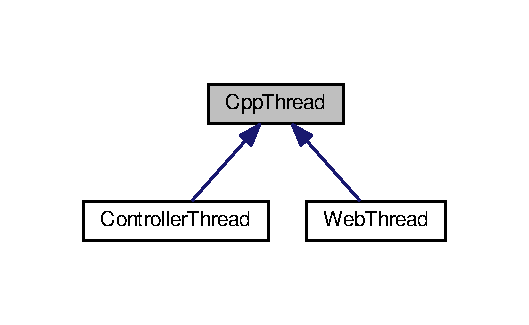
\includegraphics[width=254pt]{classCppThread__inherit__graph}
\end{center}
\end{figure}
\subsection*{Public Member Functions}
\begin{DoxyCompactItemize}
\item 
\mbox{\Hypertarget{classCppThread_a1be46d1be000f41a763289300623c609}\label{classCppThread_a1be46d1be000f41a763289300623c609}} 
void {\bfseries start} ()
\item 
\mbox{\Hypertarget{classCppThread_a8ff0fda6b913cc53764caef0e1200f3f}\label{classCppThread_a8ff0fda6b913cc53764caef0e1200f3f}} 
void {\bfseries join} ()
\item 
\mbox{\Hypertarget{classCppThread_a792b79e72250710147c452648def4a78}\label{classCppThread_a792b79e72250710147c452648def4a78}} 
virtual void {\bfseries run} ()=0
\end{DoxyCompactItemize}


\subsection{Detailed Description}
G\+NU G\+E\+N\+E\+R\+AL P\+U\+B\+L\+IC L\+I\+C\+E\+N\+SE Version 3, 29 June 2007. 

(C) 2018, Bernd Porr \href{mailto:mail@bernporr.me.uk}{\tt mail@bernporr.\+me.\+uk} 

The documentation for this class was generated from the following file\+:\begin{DoxyCompactItemize}
\item 
Classes/Cpp\+Thread.\+h\end{DoxyCompactItemize}

\hypertarget{classCppTimer}{}\section{Cpp\+Timer Class Reference}
\label{classCppTimer}\index{Cpp\+Timer@{Cpp\+Timer}}


Inheritance diagram for Cpp\+Timer\+:\nopagebreak
\begin{figure}[H]
\begin{center}
\leavevmode
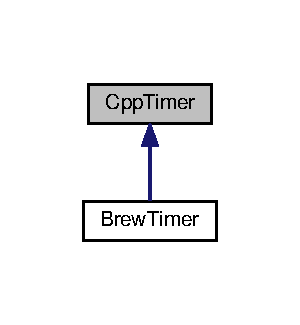
\includegraphics[width=144pt]{classCppTimer__inherit__graph}
\end{center}
\end{figure}
\subsection*{Public Member Functions}
\begin{DoxyCompactItemize}
\item 
\mbox{\Hypertarget{classCppTimer_a8d284721892e8e2665433f17045143e8}\label{classCppTimer_a8d284721892e8e2665433f17045143e8}} 
void {\bfseries start} (long nanosecs)
\item 
\mbox{\Hypertarget{classCppTimer_ac2665403595b6aee5f581d0ebfeb886c}\label{classCppTimer_ac2665403595b6aee5f581d0ebfeb886c}} 
virtual void {\bfseries timer\+Event} ()=0
\end{DoxyCompactItemize}


The documentation for this class was generated from the following file\+:\begin{DoxyCompactItemize}
\item 
Classes/Cpp\+Timer.\+h\end{DoxyCompactItemize}

\hypertarget{classDS18B20}{}\section{D\+S18\+B20 Class Reference}
\label{classDS18B20}\index{D\+S18\+B20@{D\+S18\+B20}}


Class for the digital temperature sensor \mbox{\hyperlink{classDS18B20}{D\+S18\+B20}}.  




{\ttfamily \#include $<$D\+S18\+B20.\+h$>$}



Inheritance diagram for D\+S18\+B20\+:\nopagebreak
\begin{figure}[H]
\begin{center}
\leavevmode
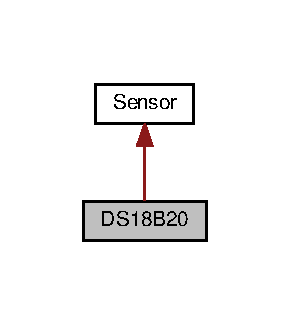
\includegraphics[width=139pt]{classDS18B20__inherit__graph}
\end{center}
\end{figure}


Collaboration diagram for D\+S18\+B20\+:\nopagebreak
\begin{figure}[H]
\begin{center}
\leavevmode
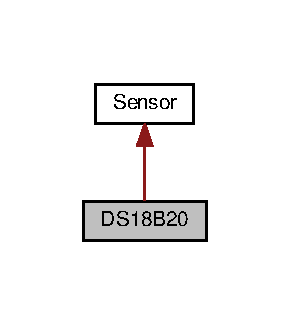
\includegraphics[width=139pt]{classDS18B20__coll__graph}
\end{center}
\end{figure}
\subsection*{Public Member Functions}
\begin{DoxyCompactItemize}
\item 
\mbox{\hyperlink{classDS18B20_af99ab621aa1603fe2dbc7ec27d387e02}{D\+S18\+B20}} (short G\+P\+IO, std\+::string dev\+\_\+id)
\begin{DoxyCompactList}\small\item\em Class constructor. \end{DoxyCompactList}\item 
void \mbox{\hyperlink{classDS18B20_ab244f4c5331b543d5e7d7bda33c54e40}{initialise}} ()
\begin{DoxyCompactList}\small\item\em Initialisation procedure. \end{DoxyCompactList}\item 
double \mbox{\hyperlink{classDS18B20_a1abd2723b34fdeb9d538476cfac4f042}{read\+Temp}} ()
\begin{DoxyCompactList}\small\item\em Read the temperature from the sensor. \end{DoxyCompactList}\end{DoxyCompactItemize}


\subsection{Detailed Description}
Class for the digital temperature sensor \mbox{\hyperlink{classDS18B20}{D\+S18\+B20}}. 



\subsection{Constructor \& Destructor Documentation}
\mbox{\Hypertarget{classDS18B20_af99ab621aa1603fe2dbc7ec27d387e02}\label{classDS18B20_af99ab621aa1603fe2dbc7ec27d387e02}} 
\index{D\+S18\+B20@{D\+S18\+B20}!D\+S18\+B20@{D\+S18\+B20}}
\index{D\+S18\+B20@{D\+S18\+B20}!D\+S18\+B20@{D\+S18\+B20}}
\subsubsection{\texorpdfstring{D\+S18\+B20()}{DS18B20()}}
{\footnotesize\ttfamily D\+S18\+B20\+::\+D\+S18\+B20 (\begin{DoxyParamCaption}\item[{short}]{G\+P\+IO,  }\item[{std\+::string}]{dev\+\_\+id }\end{DoxyParamCaption})}



Class constructor. 

Build a temperature sensor object with the pin number and the unique device ID. 
\begin{DoxyParams}{Parameters}
{\em G\+P\+IO} & pin number (wiring\+Pi convention) \\
\hline
{\em dev\+\_\+id} & device ID on the bus as a string \\
\hline
\end{DoxyParams}


\subsection{Member Function Documentation}
\mbox{\Hypertarget{classDS18B20_ab244f4c5331b543d5e7d7bda33c54e40}\label{classDS18B20_ab244f4c5331b543d5e7d7bda33c54e40}} 
\index{D\+S18\+B20@{D\+S18\+B20}!initialise@{initialise}}
\index{initialise@{initialise}!D\+S18\+B20@{D\+S18\+B20}}
\subsubsection{\texorpdfstring{initialise()}{initialise()}}
{\footnotesize\ttfamily void D\+S18\+B20\+::initialise (\begin{DoxyParamCaption}{ }\end{DoxyParamCaption})\hspace{0.3cm}{\ttfamily [virtual]}}



Initialisation procedure. 

Activates the one-\/wire interface from the Raspberry PI. 

Reimplemented from \mbox{\hyperlink{classSensor_af6f7d509e560240dfc5b1def0d87c26f}{Sensor}}.

\mbox{\Hypertarget{classDS18B20_a1abd2723b34fdeb9d538476cfac4f042}\label{classDS18B20_a1abd2723b34fdeb9d538476cfac4f042}} 
\index{D\+S18\+B20@{D\+S18\+B20}!read\+Temp@{read\+Temp}}
\index{read\+Temp@{read\+Temp}!D\+S18\+B20@{D\+S18\+B20}}
\subsubsection{\texorpdfstring{read\+Temp()}{readTemp()}}
{\footnotesize\ttfamily double D\+S18\+B20\+::read\+Temp (\begin{DoxyParamCaption}{ }\end{DoxyParamCaption})}



Read the temperature from the sensor. 

Request the temperature value from the sensor and returns a double precision value. 

The documentation for this class was generated from the following files\+:\begin{DoxyCompactItemize}
\item 
Classes/D\+S18\+B20.\+h\item 
Classes/D\+S18\+B20.\+cpp\end{DoxyCompactItemize}

\hypertarget{classSensor}{}\section{Sensor Class Reference}
\label{classSensor}\index{Sensor@{Sensor}}


A general class for simple H\+I\+G\+H/\+L\+OW sensors.  




{\ttfamily \#include $<$Sensor.\+h$>$}



Inheritance diagram for Sensor\+:\nopagebreak
\begin{figure}[H]
\begin{center}
\leavevmode
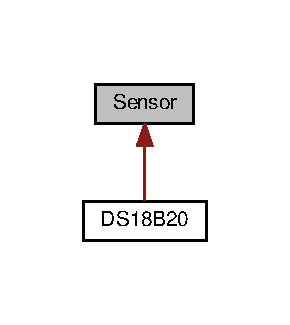
\includegraphics[width=139pt]{classSensor__inherit__graph}
\end{center}
\end{figure}
\subsection*{Public Member Functions}
\begin{DoxyCompactItemize}
\item 
\mbox{\hyperlink{classSensor_a3909b52adbe404d4ab637163001e8c86}{Sensor}} (short G\+P\+IO)
\begin{DoxyCompactList}\small\item\em Class constructor. \end{DoxyCompactList}\item 
\mbox{\Hypertarget{classSensor_af6f7d509e560240dfc5b1def0d87c26f}\label{classSensor_af6f7d509e560240dfc5b1def0d87c26f}} 
virtual void \mbox{\hyperlink{classSensor_af6f7d509e560240dfc5b1def0d87c26f}{initialise}} ()
\begin{DoxyCompactList}\small\item\em Initialisation procedure with wiring\+Pi library. \end{DoxyCompactList}\item 
\mbox{\Hypertarget{classSensor_a5d235b5abfb0446c8a5aa378630945fa}\label{classSensor_a5d235b5abfb0446c8a5aa378630945fa}} 
bool \mbox{\hyperlink{classSensor_a5d235b5abfb0446c8a5aa378630945fa}{read\+Status}} ()
\begin{DoxyCompactList}\small\item\em Reads boolean status of the sensor. \end{DoxyCompactList}\end{DoxyCompactItemize}
\subsection*{Protected Attributes}
\begin{DoxyCompactItemize}
\item 
\mbox{\Hypertarget{classSensor_ac4d08930838efb7f84ed470fa0e8979b}\label{classSensor_ac4d08930838efb7f84ed470fa0e8979b}} 
short {\bfseries pin}
\end{DoxyCompactItemize}


\subsection{Detailed Description}
A general class for simple H\+I\+G\+H/\+L\+OW sensors. 

\subsection{Constructor \& Destructor Documentation}
\mbox{\Hypertarget{classSensor_a3909b52adbe404d4ab637163001e8c86}\label{classSensor_a3909b52adbe404d4ab637163001e8c86}} 
\index{Sensor@{Sensor}!Sensor@{Sensor}}
\index{Sensor@{Sensor}!Sensor@{Sensor}}
\subsubsection{\texorpdfstring{Sensor()}{Sensor()}}
{\footnotesize\ttfamily Sensor\+::\+Sensor (\begin{DoxyParamCaption}\item[{short}]{G\+P\+IO }\end{DoxyParamCaption})}



Class constructor. 


\begin{DoxyParams}{Parameters}
{\em G\+P\+IO} & Raspberry pi pin connected to the sensor. \\
\hline
\end{DoxyParams}


The documentation for this class was generated from the following files\+:\begin{DoxyCompactItemize}
\item 
Classes/Sensor.\+h\item 
Classes/Sensor.\+cpp\end{DoxyCompactItemize}

\hypertarget{classStepper}{}\section{Stepper Class Reference}
\label{classStepper}\index{Stepper@{Stepper}}


A class to control stepper motors.  




{\ttfamily \#include $<$Stepper.\+h$>$}

\subsection*{Public Member Functions}
\begin{DoxyCompactItemize}
\item 
\mbox{\hyperlink{classStepper_a397cb4fa7c633917a0433f9455b54061}{Stepper}} (short A1, short A2, short B1, short B2, int steps)
\begin{DoxyCompactList}\small\item\em Class constructor. \end{DoxyCompactList}\item 
void \mbox{\hyperlink{classStepper_a04a7aba2471330da8f514860e6047f29}{initialise}} ()
\begin{DoxyCompactList}\small\item\em Initialisation procedure. \end{DoxyCompactList}\item 
void \mbox{\hyperlink{classStepper_a2e8ab51c08dd6773e62721460565af08}{spin}} (int speed, int revolutions, bool direction)
\begin{DoxyCompactList}\small\item\em Spin the stepper motor. \end{DoxyCompactList}\end{DoxyCompactItemize}


\subsection{Detailed Description}
A class to control stepper motors. 

This class controls general stepper motors (connected via transistor arrays) by defining each step as H\+I\+GH or L\+OW values of the coils and cycling through them after a defined interval. 

\subsection{Constructor \& Destructor Documentation}
\mbox{\Hypertarget{classStepper_a397cb4fa7c633917a0433f9455b54061}\label{classStepper_a397cb4fa7c633917a0433f9455b54061}} 
\index{Stepper@{Stepper}!Stepper@{Stepper}}
\index{Stepper@{Stepper}!Stepper@{Stepper}}
\subsubsection{\texorpdfstring{Stepper()}{Stepper()}}
{\footnotesize\ttfamily Stepper\+::\+Stepper (\begin{DoxyParamCaption}\item[{short}]{A1,  }\item[{short}]{A2,  }\item[{short}]{B1,  }\item[{short}]{B2,  }\item[{int}]{steps }\end{DoxyParamCaption})}



Class constructor. 


\begin{DoxyParams}{Parameters}
{\em A1} & First pin of the first coil \\
\hline
{\em A2} & Second pin of the first coil \\
\hline
{\em B1} & First pin of the second coil \\
\hline
{\em B2} & Second pin of the second coil \\
\hline
{\em steps} & Number of the steps of the stepper motor \\
\hline
\end{DoxyParams}


\subsection{Member Function Documentation}
\mbox{\Hypertarget{classStepper_a04a7aba2471330da8f514860e6047f29}\label{classStepper_a04a7aba2471330da8f514860e6047f29}} 
\index{Stepper@{Stepper}!initialise@{initialise}}
\index{initialise@{initialise}!Stepper@{Stepper}}
\subsubsection{\texorpdfstring{initialise()}{initialise()}}
{\footnotesize\ttfamily void Stepper\+::initialise (\begin{DoxyParamCaption}{ }\end{DoxyParamCaption})}



Initialisation procedure. 

Function required to initialise the stepper motor to wiring\+Pi standards. \mbox{\Hypertarget{classStepper_a2e8ab51c08dd6773e62721460565af08}\label{classStepper_a2e8ab51c08dd6773e62721460565af08}} 
\index{Stepper@{Stepper}!spin@{spin}}
\index{spin@{spin}!Stepper@{Stepper}}
\subsubsection{\texorpdfstring{spin()}{spin()}}
{\footnotesize\ttfamily void Stepper\+::spin (\begin{DoxyParamCaption}\item[{int}]{speed,  }\item[{int}]{revolutions,  }\item[{bool}]{direction }\end{DoxyParamCaption})}



Spin the stepper motor. 

Spin the stepper motor in a certain direction and at a certain speed as defined by the input parameters. 
\begin{DoxyParams}{Parameters}
{\em speed} & spinning speed \\
\hline
{\em revolutions} & number of revolutions  clockwise or anti-\/clockwise direction specified as a boolean value. \\
\hline
\end{DoxyParams}


The documentation for this class was generated from the following files\+:\begin{DoxyCompactItemize}
\item 
Classes/Stepper.\+h\item 
Classes/Stepper.\+cpp\end{DoxyCompactItemize}

\hypertarget{classTea}{}\section{Tea Class Reference}
\label{classTea}\index{Tea@{Tea}}


A class defining a type of tea by its brewing time and temperature.  




{\ttfamily \#include $<$Tea.\+h$>$}

\subsection*{Public Member Functions}
\begin{DoxyCompactItemize}
\item 
\mbox{\hyperlink{classTea_a0788a36a50457565433259205e916f04}{Tea}} (double brew\+\_\+temp, double brew\+\_\+time)
\begin{DoxyCompactList}\small\item\em Class constructor. \end{DoxyCompactList}\item 
void \mbox{\hyperlink{classTea_acb5bec6356db757e2deb5598b6a7ad37}{set\+Brew\+Temperature}} (double temp)
\begin{DoxyCompactList}\small\item\em Set the brewing temperature. \end{DoxyCompactList}\item 
void \mbox{\hyperlink{classTea_a3f9bb73bd2d9978b63f1dd1a2463f025}{set\+Brew\+Time}} (double time)
\begin{DoxyCompactList}\small\item\em Set the brewing time. \end{DoxyCompactList}\item 
\mbox{\Hypertarget{classTea_ac4a33558dad77fc196da4eb8ca5ea80b}\label{classTea_ac4a33558dad77fc196da4eb8ca5ea80b}} 
double \mbox{\hyperlink{classTea_ac4a33558dad77fc196da4eb8ca5ea80b}{get\+Brew\+Temperature}} ()
\begin{DoxyCompactList}\small\item\em Read the brewing temperature. \end{DoxyCompactList}\item 
\mbox{\Hypertarget{classTea_a9b95d6c5fc91c1bb26a125a8fb8d0e32}\label{classTea_a9b95d6c5fc91c1bb26a125a8fb8d0e32}} 
double \mbox{\hyperlink{classTea_a9b95d6c5fc91c1bb26a125a8fb8d0e32}{get\+Brew\+Time}} ()
\begin{DoxyCompactList}\small\item\em Read the brewing time. \end{DoxyCompactList}\end{DoxyCompactItemize}


\subsection{Detailed Description}
A class defining a type of tea by its brewing time and temperature. 

Define a tea object in the context of Excellentea in terms of its brewing time and temperature. 

\subsection{Constructor \& Destructor Documentation}
\mbox{\Hypertarget{classTea_a0788a36a50457565433259205e916f04}\label{classTea_a0788a36a50457565433259205e916f04}} 
\index{Tea@{Tea}!Tea@{Tea}}
\index{Tea@{Tea}!Tea@{Tea}}
\subsubsection{\texorpdfstring{Tea()}{Tea()}}
{\footnotesize\ttfamily Tea\+::\+Tea (\begin{DoxyParamCaption}\item[{double}]{brew\+\_\+temp,  }\item[{double}]{brew\+\_\+time }\end{DoxyParamCaption})}



Class constructor. 

Create a tea object. 
\begin{DoxyParams}{Parameters}
{\em brew\+\_\+temp} & Brewing temperature in °C. \\
\hline
{\em brew\+\_\+time} & Brewing time in minutes. \\
\hline
\end{DoxyParams}


\subsection{Member Function Documentation}
\mbox{\Hypertarget{classTea_acb5bec6356db757e2deb5598b6a7ad37}\label{classTea_acb5bec6356db757e2deb5598b6a7ad37}} 
\index{Tea@{Tea}!set\+Brew\+Temperature@{set\+Brew\+Temperature}}
\index{set\+Brew\+Temperature@{set\+Brew\+Temperature}!Tea@{Tea}}
\subsubsection{\texorpdfstring{set\+Brew\+Temperature()}{setBrewTemperature()}}
{\footnotesize\ttfamily void Tea\+::set\+Brew\+Temperature (\begin{DoxyParamCaption}\item[{double}]{temp }\end{DoxyParamCaption})}



Set the brewing temperature. 


\begin{DoxyParams}{Parameters}
{\em temp} & Brewing temperature in °C. \\
\hline
\end{DoxyParams}
\mbox{\Hypertarget{classTea_a3f9bb73bd2d9978b63f1dd1a2463f025}\label{classTea_a3f9bb73bd2d9978b63f1dd1a2463f025}} 
\index{Tea@{Tea}!set\+Brew\+Time@{set\+Brew\+Time}}
\index{set\+Brew\+Time@{set\+Brew\+Time}!Tea@{Tea}}
\subsubsection{\texorpdfstring{set\+Brew\+Time()}{setBrewTime()}}
{\footnotesize\ttfamily void Tea\+::set\+Brew\+Time (\begin{DoxyParamCaption}\item[{double}]{time }\end{DoxyParamCaption})}



Set the brewing time. 


\begin{DoxyParams}{Parameters}
{\em time} & Brewing time in minutes. \\
\hline
\end{DoxyParams}


The documentation for this class was generated from the following files\+:\begin{DoxyCompactItemize}
\item 
Classes/Tea.\+h\item 
Classes/Tea.\+cpp\end{DoxyCompactItemize}

\hypertarget{classWebThread}{}\section{Web\+Thread Class Reference}
\label{classWebThread}\index{Web\+Thread@{Web\+Thread}}


A thread that handles the web interface.  




{\ttfamily \#include $<$Web\+Thread.\+h$>$}



Inheritance diagram for Web\+Thread\+:\nopagebreak
\begin{figure}[H]
\begin{center}
\leavevmode
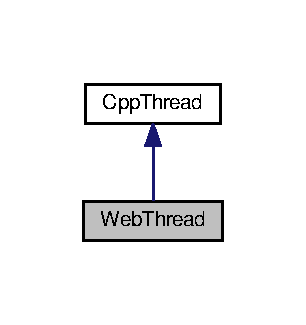
\includegraphics[width=147pt]{classWebThread__inherit__graph}
\end{center}
\end{figure}


Collaboration diagram for Web\+Thread\+:\nopagebreak
\begin{figure}[H]
\begin{center}
\leavevmode
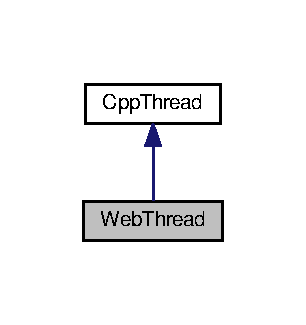
\includegraphics[width=147pt]{classWebThread__coll__graph}
\end{center}
\end{figure}
\subsection*{Public Member Functions}
\begin{DoxyCompactItemize}
\item 
\mbox{\Hypertarget{classWebThread_a72ae681bcec8cabcd4738ec819c03261}\label{classWebThread_a72ae681bcec8cabcd4738ec819c03261}} 
\mbox{\hyperlink{classWebThread_a72ae681bcec8cabcd4738ec819c03261}{Web\+Thread}} ()
\begin{DoxyCompactList}\small\item\em Class constructor. \end{DoxyCompactList}\end{DoxyCompactItemize}


\subsection{Detailed Description}
A thread that handles the web interface. 

The documentation for this class was generated from the following files\+:\begin{DoxyCompactItemize}
\item 
Classes/Web\+Thread.\+h\item 
Classes/Web\+Thread.\+cpp\end{DoxyCompactItemize}

%--- End generated contents ---

% Index
\backmatter
\newpage
\phantomsection
\clearemptydoublepage
\addcontentsline{toc}{chapter}{Index}
\printindex

\end{document}
